\label{sec:dp-calib-pns-alt}

\subsubsection{Small Format Moderator}
An alternative method for delivering the neutrons is to use the existing calibration feedthroughs. In the current cryostat design, \num{20} calibration feedthroughs with a \SI{25}{\cm} outer diameter will be available on top of the cryostat. One can design the neutron source with an ultra-thin $DD$ generator that fits the size of the feedthrough as shown in Figure~\ref{fig:PNS_Two_Designs} (right). The problem is that there will be no space in the feedthrough for the shielding materials to fit in, so additional shielding will need to be placed around the feedthrough. The weight of this compact neutron source will be about \SI{140}{\kg}, so minimal special mounting is needed. In addition, the source may be moved as well, allowing further flexibility. The effective neutron flux is expected to be similar to that of the baseline deployment. 

\begin{dunefigure}[\dshort{pns} two designs]{fig:PNS_Two_Designs}
{(right) Small format neutron source deployed inside the calibration feedthrough ports. (left) For comparison, large format neutron source deployed above/inside the human access ports is shown on the left.}
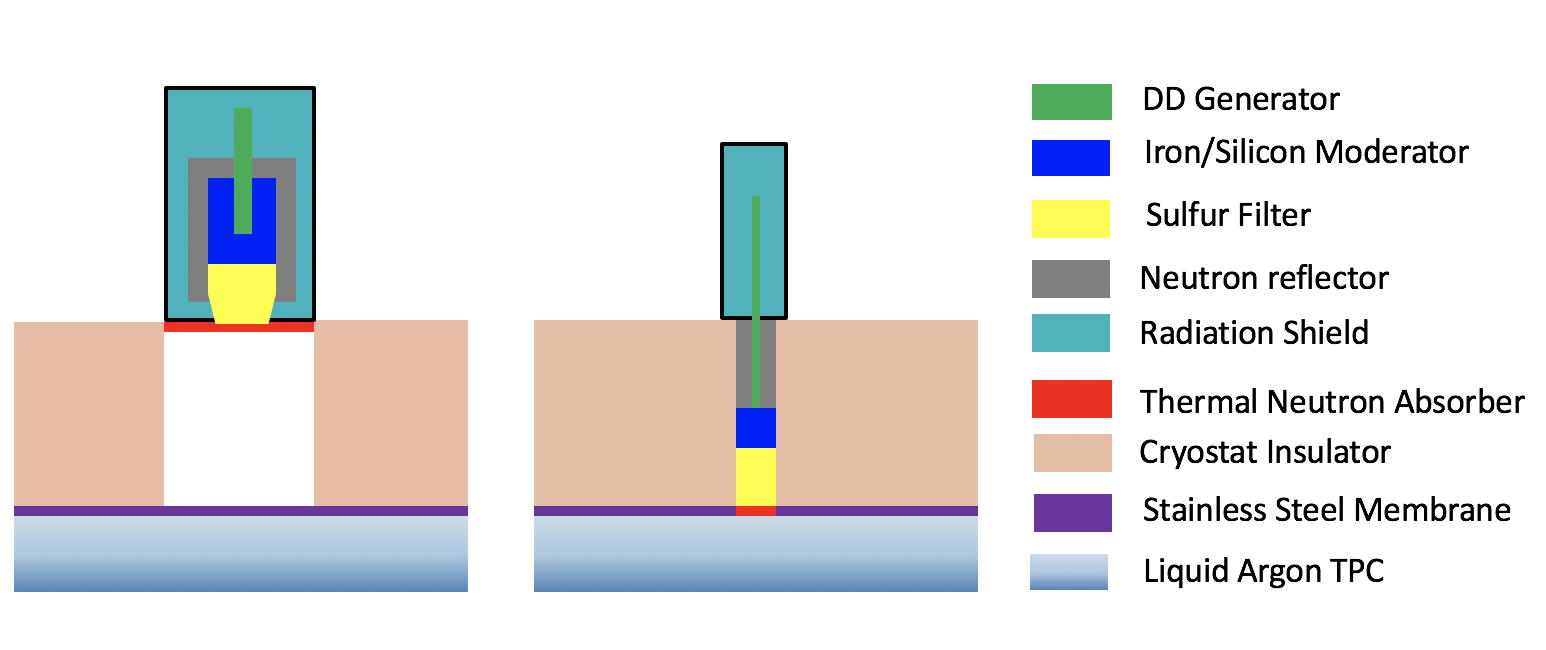
\includegraphics[width=16cm]{graphics/PNS_Moderator_Combined.png}
\end{dunefigure}

The volume coverage at the center of the detector can be significantly increased by using a small format neutron source deployed on top at the center of the cryostat using the multi-purpose feedthroughs.  
Figure~\ref{fig:PNS_alternative_ncap} shows the position distribution of the neutron captures using two large format sources at the corner human access ports and one additional small format source in the middle of the cryostat. The small format source is %essential 
important to complement the coverage at the center of the TPC. The alternative small format neutron source is very compact and lightweight, so further coverage improvement is possible by moving the source to different calibration feedthroughs. The deployment of the small format source would require sharing of the feedthrough ports with other calibration systems, which is currently under investigation.

\begin{dunefigure}[Pulsed neutron system neutron capture positions inside a \dshort{dune}-sized \dshort{tpc}]{fig:PNS_alternative_ncap}
{Neutron capture positions inside a \dword{dune}-sized \dword{tpc}, assuming alternative configuration with two large format neutron sources located at the corner human access ports and one small format neutron source located at the center of the cryostat, which compensates the missing volume coverage of the two large format sources at the center of the detector.  $L$=\SI{60}{\m} (along $Z$ axis, horizontally parallel to the beam direction), $W$=\SI{14.5}{\m} (along $X$ axis, horizontally perpendicular to the beam direction), $H$=\SI{10}{\m} (along $Y$ axis, vertically perpendicular to the beam direction). \num{2.7e7} $DD$ generator neutrons with \SI{2.5}{\MeV} energy were simulated in each moderator and propagated inside the \dword{tpc}. Top (left) and side (right) views of neutron capture positions are shown.}
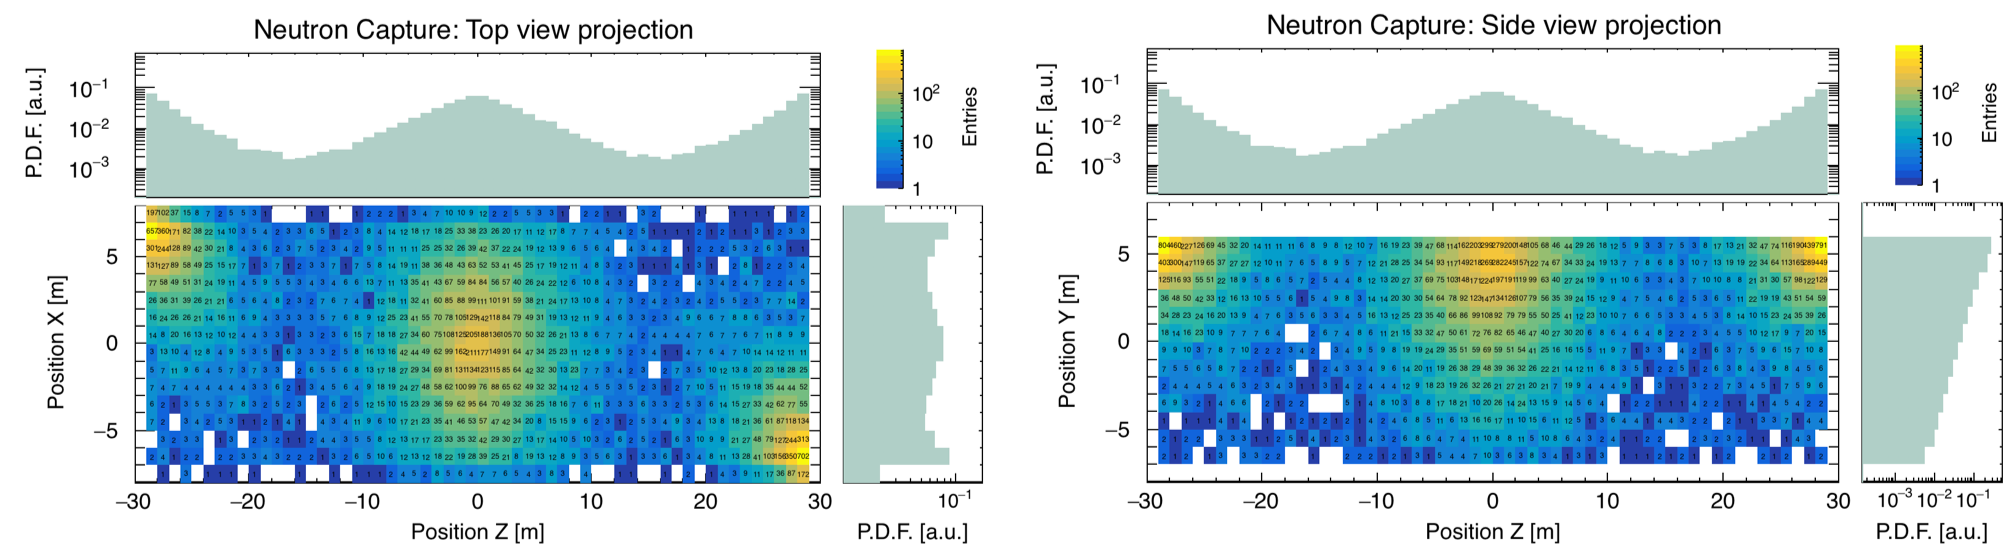
\includegraphics[width=18cm]{graphics/PNS_ncapDistribution_three_sources.png}
%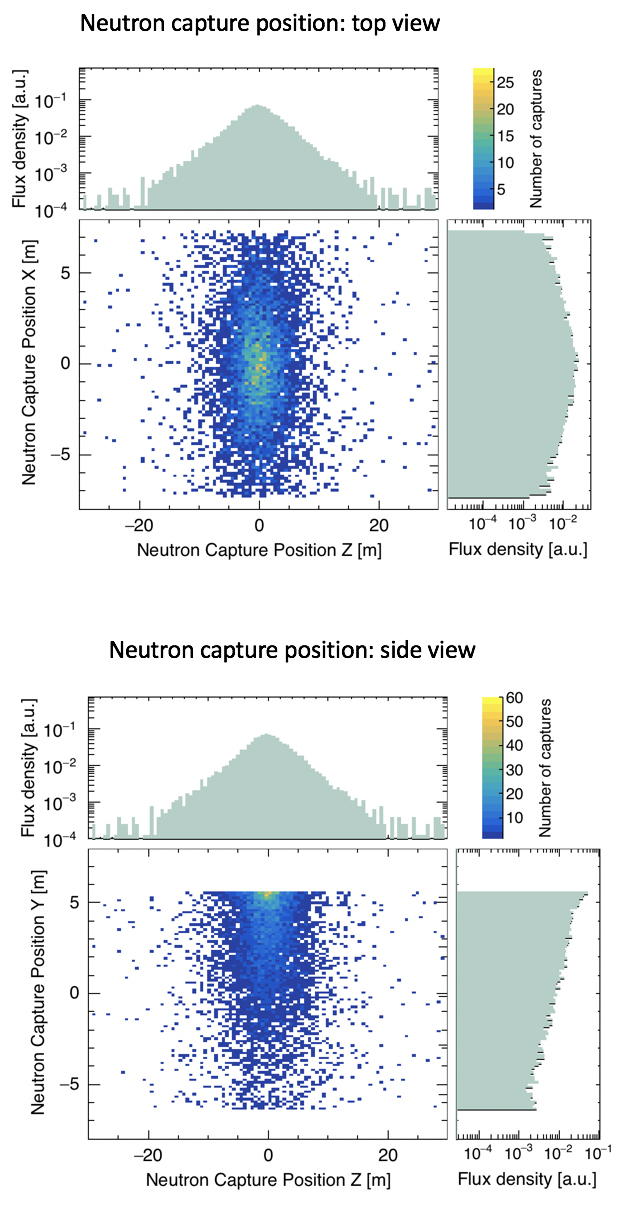
\includegraphics[width=10cm]{graphics/PNS_NcapPosition_v2.png}
\end{dunefigure}

In principle, for the baseline deployment plan as shown in Figure~\ref{fig:PNS_ncapDistribution_two_sources}, we can run the neutron source for a longer time to increase the coverage at the central region of the detector. However, this would result in a huge data volume. So, the best way to complement the coverage at the center of the detector is to use the alternate deployment as discussed here. This design would require a total number of \num{4600} pulses to calibrate the entire \nominalmodsize module. Assuming that three neutron sources with identical neutron capture yield are operated in synchronization mode, \num{1500} triggers are needed for each calibration run. Therefore, the total data volume per run would be 

\begin{equation}
\num{1500}~{\rm Triggers} \times \num{1.5}~{\rm Bytes}\times
\SI{2}{\mega\hertz}\times \SI{5.4}{\milli\s}\times \num{384000}~{\rm channels} = \num{9.5}~{\rm TB/run}.
\end{equation}

The recommended trigger rate of the \dword{pns} system is \SI{0.5}{\hertz} which is limited by the bandwidth of the DAQ event builder. Assuming that the spatial distribution of the neutron capture is uniform across the whole detector volume, the operation time per calibration run would be \num{50} minutes.   
Running the \dword{pns} calibration system twice a year would result in a total data volume of \SI{19}{TB} per \nominalmodsize per year. 
For realistic neutron capture distribution that is non-uniform, we expected to operate the \dword{pns} system for a period of 10 times longer than that under the ideal assumption (9.5 TB/run). As a result, the data size per calibration run would be 95 TB/run and running the PNS calibration twice a year would result in a total data size of 190 TB/year and four times a year would result in 380 TB/year.